% Q20: source PDF p3; only BA and BC, AB is not a diameter.
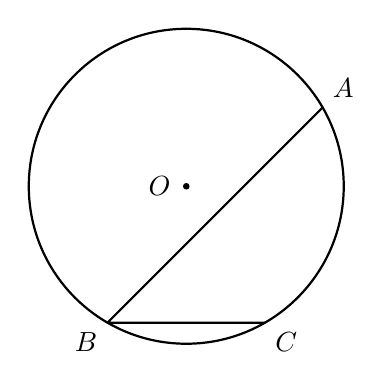
\begin{tikzpicture}[line cap=round,line join=round,thick]
\coordinate (O) at (0,0);
\coordinate (A) at (30:2); \coordinate (B) at (240:2); \coordinate (C) at (300:2);
\draw (O) circle[radius=2]; \draw (A)--(B)--(C);
\fill (O) circle[radius=1.2pt]; \node[left=2pt] at (O) {$O$};
\node[above right] at (A) {$A$}; \node[below left] at (B) {$B$};
\node[below right] at (C) {$C$};
\end{tikzpicture}
